\section{Stopped Proton}
\label{Sec:Proton}

%
%Proton events are applied following simple selections.
Proton event selection
\begin{itemize}
\item Protons are selected by the information of beam counters.
\item Drift time of the hit at the injection point: 150$mu$s to 300$\mu$s which corresponds with T32 BDC fiducial volume.
\item Total number of hits in the cluster is greater than 5.
%\item Only one hit are required at the same channel in the cluster to remove multi-track events.
\item Only one cluster in the event
\end{itemize}

For good proton events, we compare each parameter between data and MC.
Figure\ref{fig:various_distribution} shows the comparison of the distribution of 
Hit Charge, Hit Sigma, Stopped Channel and  Cluster Charge between data and MC.
All four distributions of MC reproduce data well.
Especially, the agreement of stopped channel distribution shows the consistent 
the momentum estimation by TOF information with the initial momentum of the particles injected to 250L detector.\\

\begin{figure}[htbp]
  \centering
  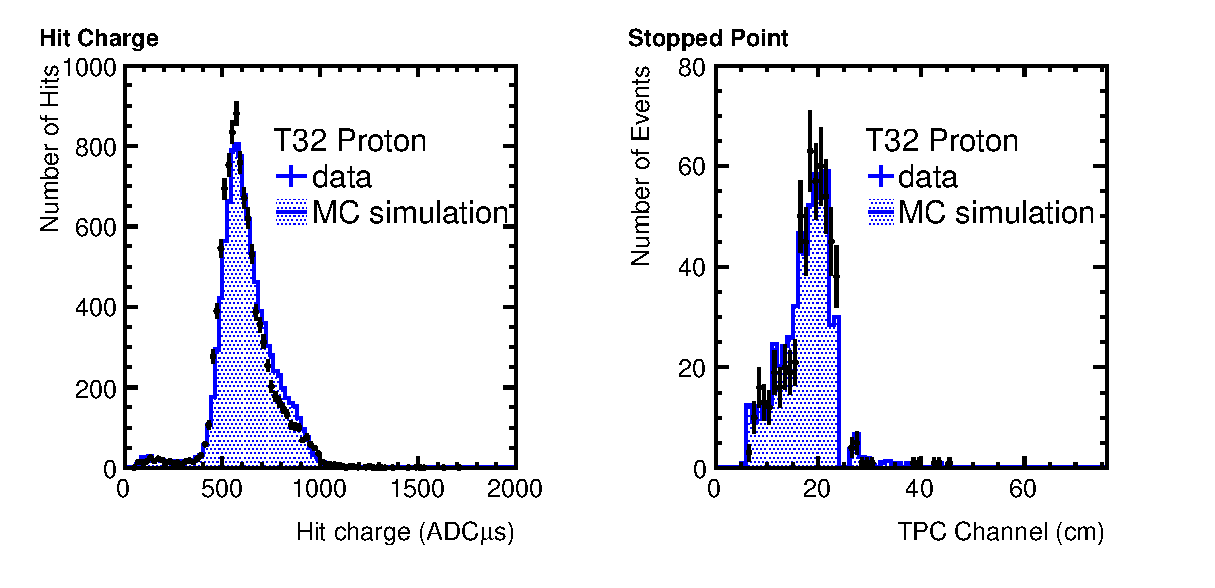
\includegraphics[width=1.0\hsize,clip]{./fig/Proton_1.eps}
  \caption{Hit Charge, Hit Sigma, Stopped Channel, Cluster Charge}
  \label{fig:various_distribution}
\end{figure}

Figure\ref{fig:ADC_distribution} shows the hit charge distribution of each distance from stopped point.
Hit charge distributions of MC simulation are good agreements with data.
Figure\ref{fig:Mean_comparison} shows the mean of the hit charge distribution of each distance from stopped point.
%Figure\ref{fig:Mean_comparison_ratio} shows the ratios of Data/MC.
%The ratios are within 94\%$\sim$105\%.
MC simulation reproduce the charge response of data in high and wide dE/dx region well.

\begin{figure}[htbp]
  \centering
  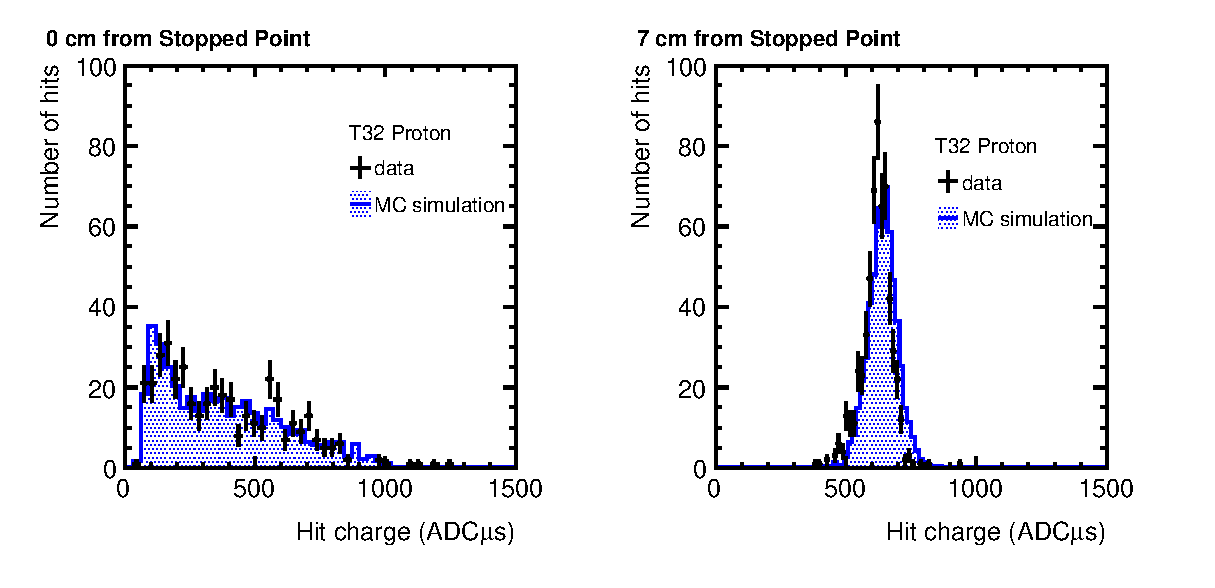
\includegraphics[width=1.0\hsize,clip]{fig/Proton_2.eps}
  \caption{Hit charge distribution of each distance from stopped point}
  \label{fig:ADC_distribution}
\end{figure}

%\begin{figure}[htbp]
%  \begin{center}
%  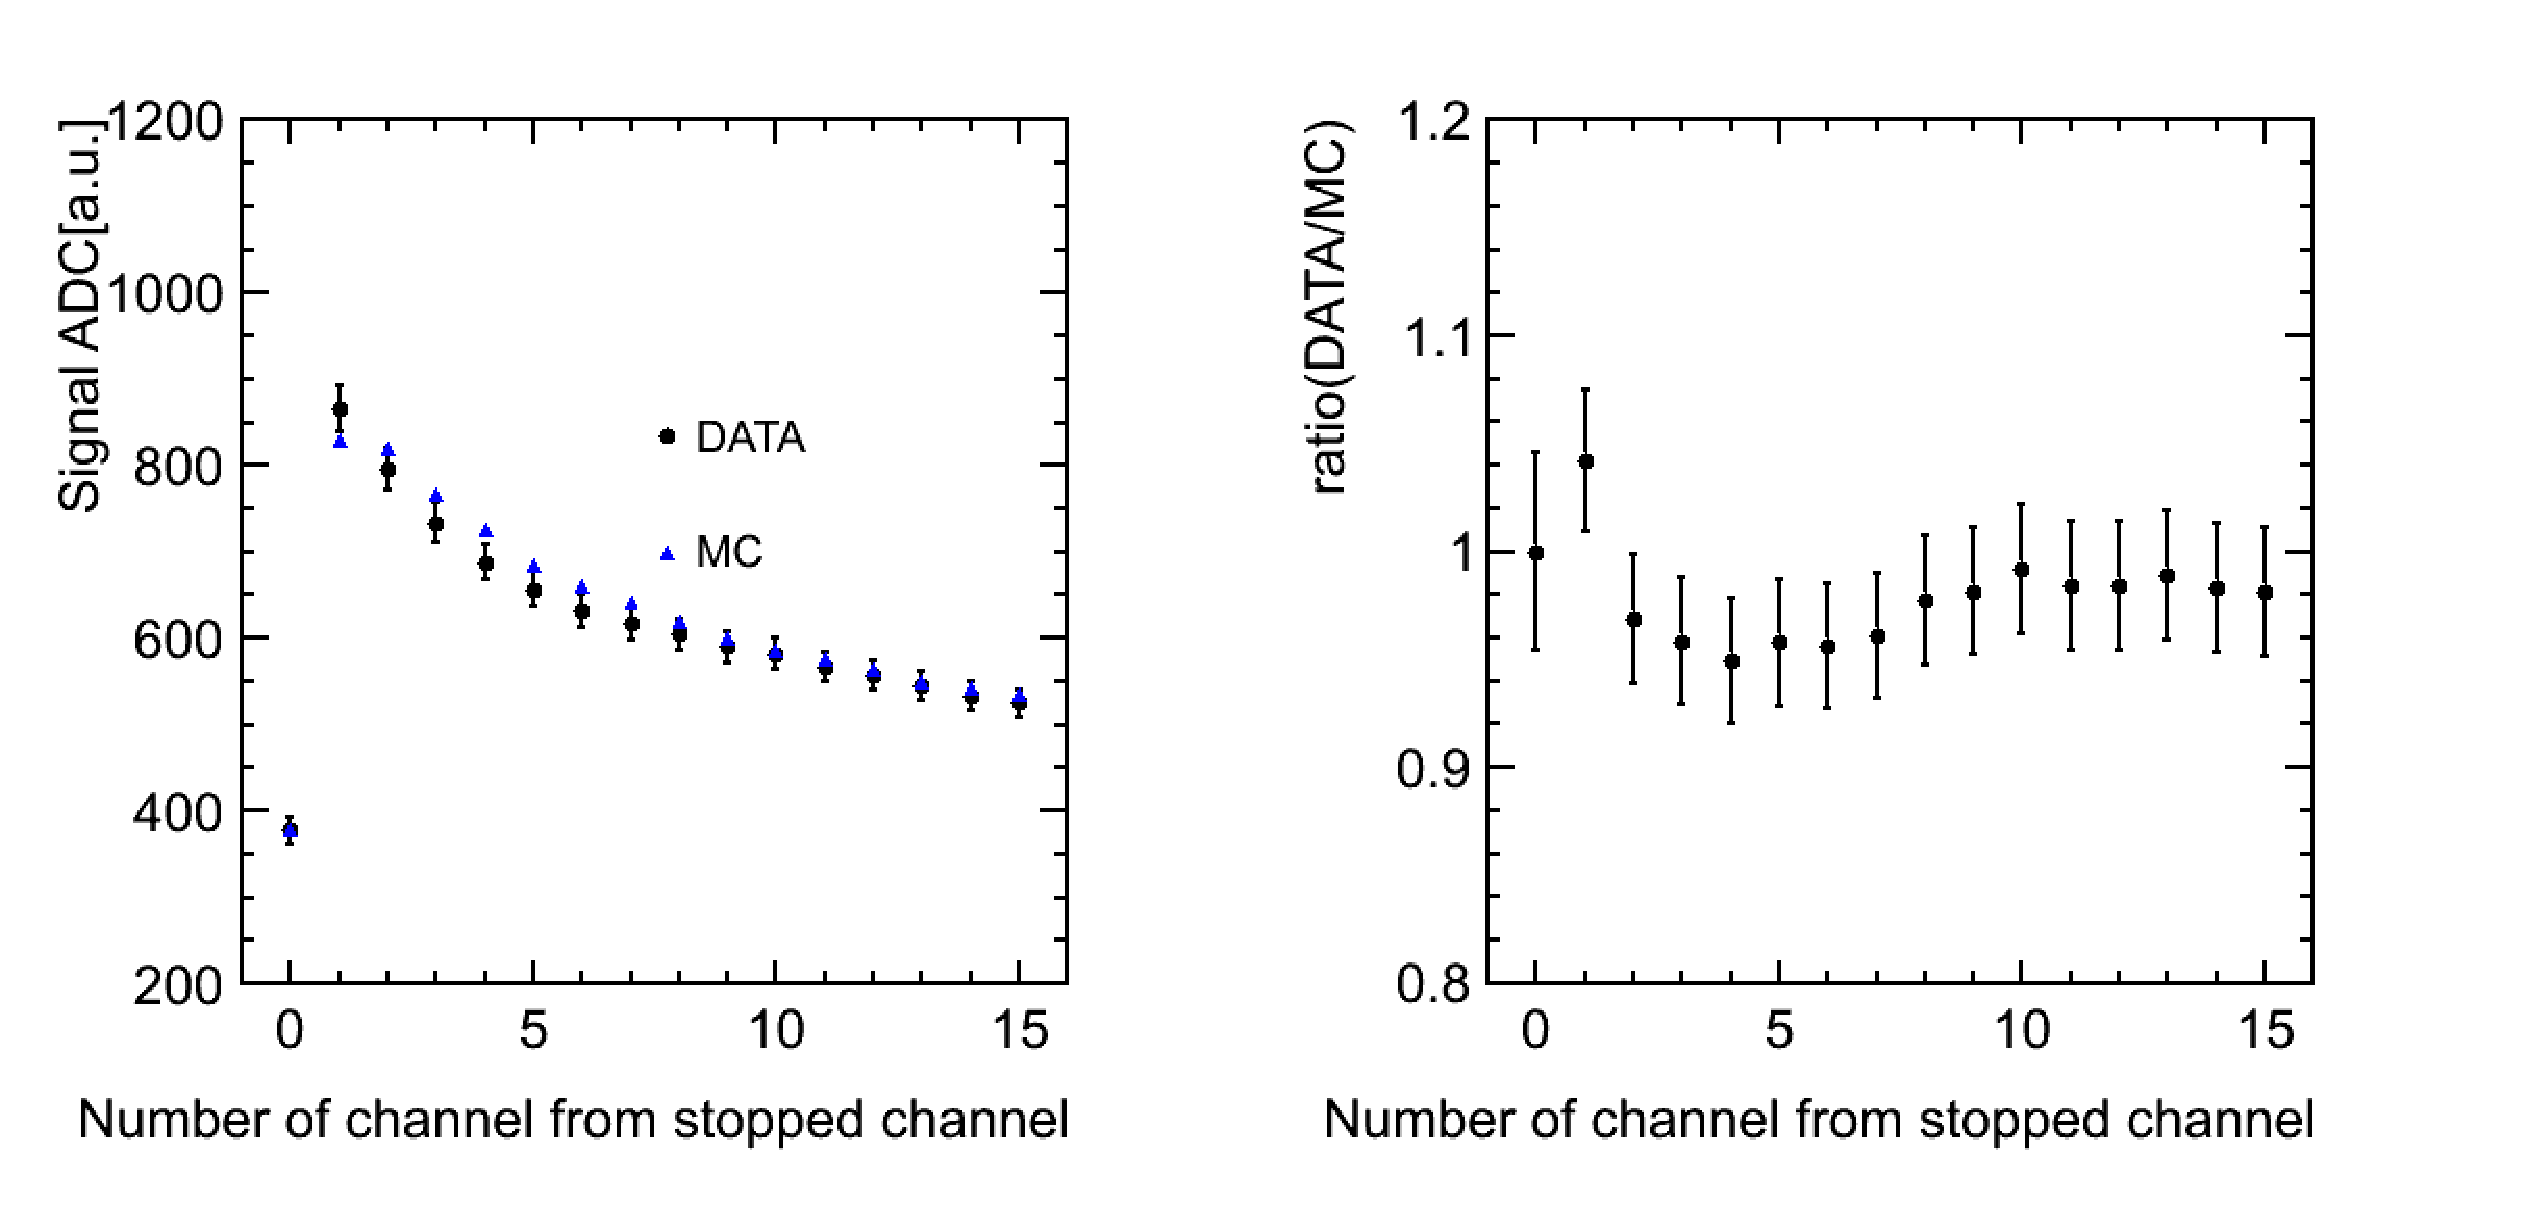
\includegraphics[width=1.0\hsize,clip]{fig/stop_proton3.eps}
%  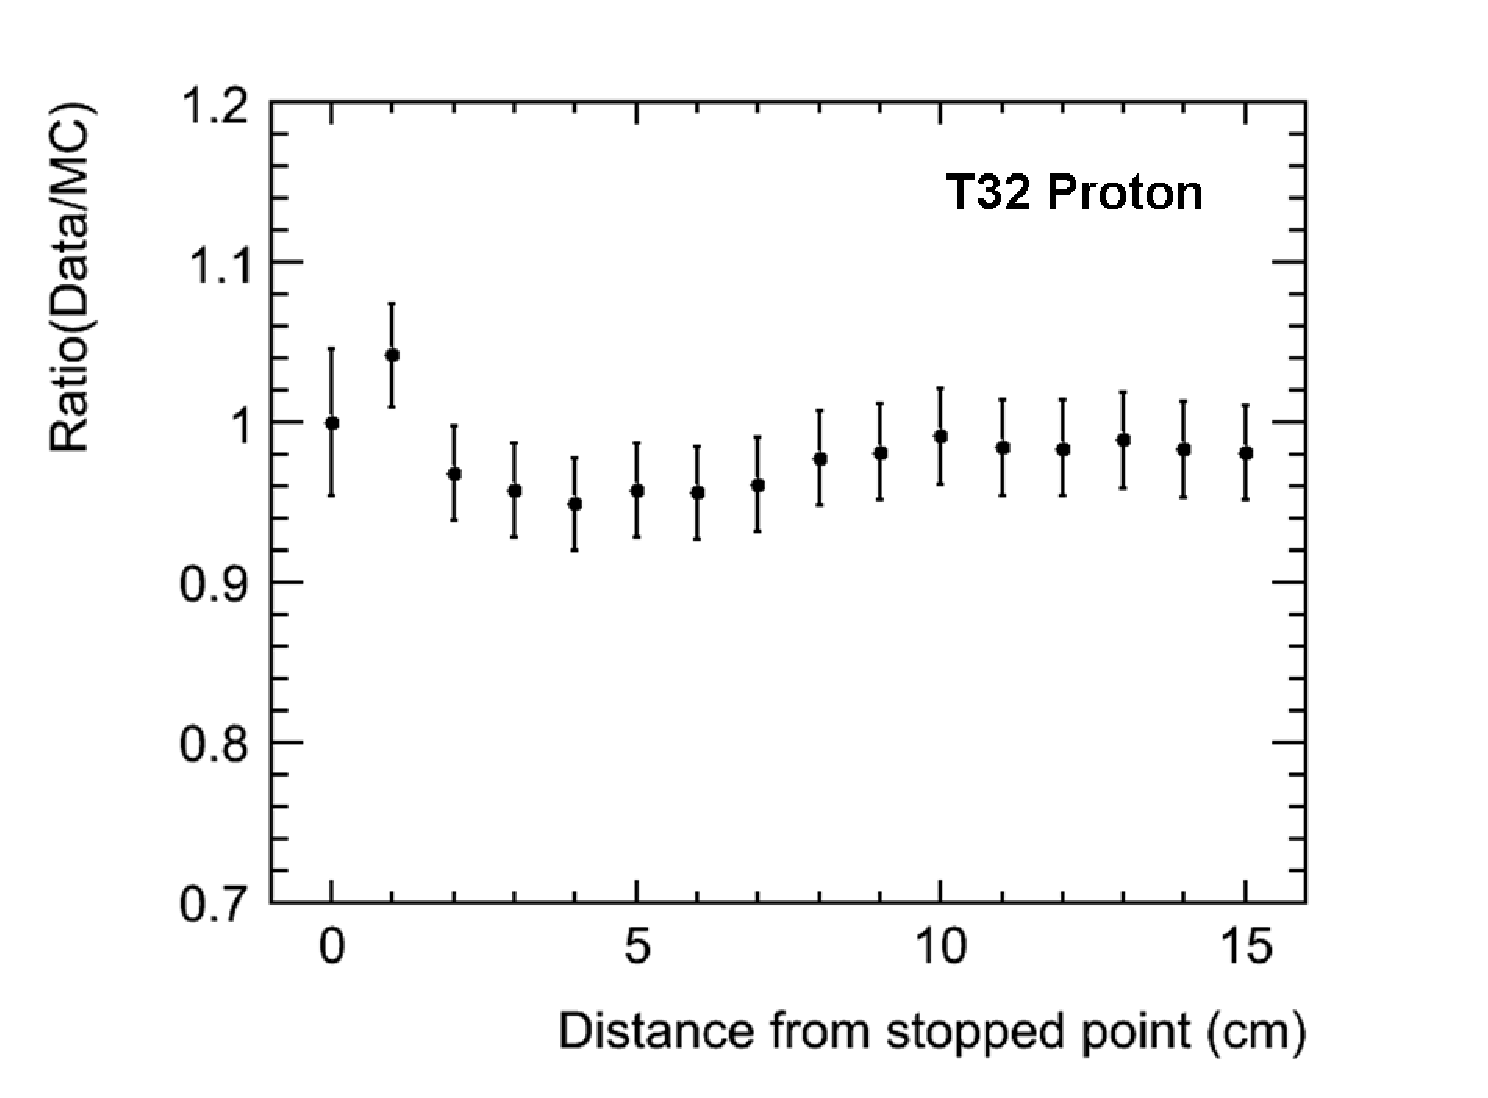
\includegraphics[width=0.8\hsize,clip]{fig/stop_proton4.eps}
%  \end{center}
%  \caption{Data-MC comparison of the mean of hit charge distribution}
%  \label{fig:Mean_comparison}
%  \label{fig:Mean_comparison_ratio}
%\end{figure}

% LocalWords:  fiducial

